\documentclass[11pt,a4paper]{article}

\usepackage[a4paper,top=22mm,bottom=24mm,left=23mm,right=23mm,headheight=22pt]{geometry}
\usepackage[T1]{fontenc}
\usepackage{lmodern}
\usepackage{amsmath,amssymb}
\usepackage{microtype}
\usepackage[table]{xcolor}
\definecolor{Primary}{HTML}{174A72}
\definecolor{Secondary}{HTML}{2D6A8A}
\definecolor{LightBlue}{HTML}{EAF3F8}
\definecolor{RuleGray}{HTML}{CBD5E1}
\definecolor{TextGray}{HTML}{475569}

\usepackage{graphicx}
\graphicspath{{figures/}}
\usepackage{longtable,array,tabularx}
\usepackage{calc}
\usepackage{etoolbox}
\usepackage{enumitem}
\usepackage{titlesec}
\usepackage{fancyhdr}
\usepackage[most]{tcolorbox}
\usepackage{tikz}
\usetikzlibrary{arrows.meta,positioning,shapes.geometric}
\usepackage{caption}
\usepackage{float}
\usepackage{pdflscape}
\usepackage{hyperref}
\usepackage{bookmark}
\usepackage{xurl}
\usepackage{soul}

\hypersetup{
  colorlinks=true,
  linkcolor=Primary,
  urlcolor=Secondary,
  citecolor=Primary,
  pdftitle={Flood-Affected Village Mapping},
  pdfsubject={Satellite Imagery, GNSS and GIS-Based Assessment},
  pdfauthor={Academic Assignment}
}
\urlstyle{same}

\setlength{\parindent}{0pt}
\setlength{\parskip}{5.5pt plus 1.5pt minus 1pt}
\setlength{\emergencystretch}{3em}
\setcounter{secnumdepth}{-\maxdimen}
\setcounter{tocdepth}{2}
\renewcommand{\contentsname}{Contents}
\renewcommand{\arraystretch}{1.18}
\providecommand{\tightlist}{\setlength{\itemsep}{2pt}\setlength{\parskip}{0pt}}
\newcommand{\real}[1]{#1}
\setlength{\arrayrulewidth}{0.45pt}
\arrayrulecolor{RuleGray}

\setlist[itemize]{leftmargin=1.7em,itemsep=3pt,topsep=3pt}
\setlist[enumerate]{leftmargin=1.9em,itemsep=3pt,topsep=3pt}

\titleformat{\section}
  {\Large\bfseries\sffamily\color{Primary}}
  {}{0pt}{}
  [\vspace{1mm}\color{RuleGray}\titlerule]
\titleformat{\subsection}
  {\large\bfseries\sffamily\color{Secondary}}
  {}{0pt}{}
\titleformat{\subsubsection}
  {\normalsize\bfseries\sffamily\color{TextGray}}
  {}{0pt}{}
\titlespacing*{\section}{0pt}{16pt}{8pt}
\titlespacing*{\subsection}{0pt}{12pt}{5pt}
\titlespacing*{\subsubsection}{0pt}{9pt}{3pt}

\pagestyle{fancy}
\fancyhf{}
\fancyhead[L]{\sffamily\small\color{TextGray}Flood-Affected Village Mapping}
\fancyhead[R]{\sffamily\small\color{TextGray}Satellite Imagery, GNSS and GIS}
\fancyfoot[C]{\sffamily\small\thepage}
\renewcommand{\headrulewidth}{0.4pt}
\renewcommand{\headrule}{\hbox to\headwidth{\color{RuleGray}\leaders\hrule height \headrulewidth\hfill}}

\AtBeginEnvironment{longtable}{\small\setlength{\tabcolsep}{4pt}\renewcommand{\arraystretch}{1.28}}
\makeatletter
\patchcmd\longtable{\par}{\if@noskipsec\mbox{}\fi\par}{}{}
\makeatother

\newtcolorbox{summarybox}{
  enhanced,
  breakable,
  colback=LightBlue,
  colframe=Primary,
  boxrule=0.7pt,
  arc=2mm,
  left=4mm,right=4mm,top=3mm,bottom=3mm
}

\captionsetup{
  font=small,
  labelfont={bf,sf,color=Primary},
  textfont={color=TextGray},
  justification=centering,
  skip=5pt
}

\tikzset{
  flownode/.style={
    draw=Primary,
    fill=LightBlue,
    rounded corners=2mm,
    minimum height=12mm,
    text width=33mm,
    align=center,
    font=\footnotesize\sffamily\bfseries,
    text=Primary
  },
  flowarrow/.style={
    -{Stealth[length=2.5mm]},
    line width=0.8pt,
    draw=Secondary
  }
}

\begin{document}
\hypersetup{pageanchor=false}

\begin{titlepage}
\thispagestyle{empty}
\centering
\vspace*{18mm}
{\sffamily\bfseries\fontsize{25}{30}\selectfont\color{Primary} FLOOD-AFFECTED\\[2mm] VILLAGE MAPPING\par}
\vspace{6mm}
{\sffamily\Large\color{Secondary}Satellite Imagery, GNSS and GIS-Based Assessment\par}
\vspace{8mm}
{\color{Primary}\rule{0.72\textwidth}{1.2pt}\par}
\vspace{16mm}
\begin{summarybox}
\centering
{\sffamily\large\bfseries Assignment Report}\par
\vspace{2mm}
A district-level framework for identifying flood-affected villages after heavy rainfall using satellite remote sensing, spatial analysis, GNSS field validation and GIS-based early warning.
\end{summarybox}
\vfill
\begin{tabularx}{0.82\textwidth}{>{\bfseries\sffamily}l X}
Name & \rule{0.98\linewidth}{0.4pt}\\[6mm]
Register Number & \rule{0.98\linewidth}{0.4pt}\\[6mm]
Course / Subject & \rule{0.98\linewidth}{0.4pt}\\[6mm]
Institution & \rule{0.98\linewidth}{0.4pt}\\[6mm]
Date & 30 July 2026\\
\end{tabularx}
\vfill
{\sffamily\small\color{TextGray}Prepared for academic submission\par}
\end{titlepage}

\hypersetup{pageanchor=true}
\pagenumbering{roman}
\tableofcontents
\clearpage
\pagenumbering{arabic}

\section{Executive Summary}\label{executive-summary}

Heavy rainfall can inundate large areas within hours, cut road access, isolate settlements and make conventional field surveys slow or unsafe. Satellite imagery gives district administrators a synoptic and repeatable view of flood extent, while GIS converts the detected water into actionable village-level information. For monsoon emergencies, Synthetic Aperture Radar (SAR) imagery is the most dependable observation source because it works through clouds and at night. Optical imagery remains valuable for detailed visual interpretation, spectral water indices and post-event damage assessment when cloud-free scenes are available. The recommended operational approach is therefore a multi-sensor workflow: use Sentinel-1 or comparable SAR for rapid inundation extraction; use Sentinel-2, Landsat or high-resolution optical data for confirmation; integrate a digital elevation model, permanent-water mask, rainfall, river-gauge observations, roads, buildings, population and village boundaries; and validate critical locations using GNSS-tagged field observations.

The proposed early-warning framework continuously combines satellite rainfall and weather imagery, automated river and rain gauges, GNSS positioning, hydrologic and hydraulic models, and a district GIS dashboard. Threshold-based and model-based alerts are issued at watch, warning and evacuation levels. The system should not treat a satellite flood map as perfect ground truth: uncertainty, sensor limitations, vegetation, urban radar effects, cloud contamination and acquisition delays must be communicated explicitly. The final administrative products are a flood-inundation map, an affected-village table, exposure estimates, safe-route and shelter maps, a prioritized field-verification plan and time-stamped alert messages.

\begin{summarybox}
{\sffamily\bfseries\color{Primary}Recommended operational principle}\par
Use SAR first for detection, optical imagery second for confirmation, terrain and permanent-water data for error reduction, and GNSS field observations for validation. Publish both the mapped flood extent and an uncertainty/confidence layer.
\end{summarybox}

\section{1. Introduction and Objectives}\label{introduction-and-objectives}

Flood mapping is the process of identifying the spatial extent, timing and, where possible, depth of water outside its normal river, lake or reservoir boundary. In a district-administration context, the practical question is not only "Where is water?" but also "Which villages, roads, crops, public facilities and populations are affected, and what should be prioritized?" Satellite remote sensing is suited to this task because the same sensor can repeatedly observe a wide area, measurements are georeferenced, and historical scenes can be compared with post-rainfall conditions.

This assignment addresses five objectives:

\begin{itemize}
\item
  Analyze the advantages and limitations of satellite imagery for flood mapping.
\item
  Compare radar, optical and meteorological satellite datasets for operational flood monitoring.
\item
  Design an end-to-end GIS workflow that converts satellite observations into affected-village information.
\item
  Recommend preprocessing, classification, change-detection and data-fusion techniques that improve accuracy.
\item
  Propose an early-warning framework that integrates satellite imagery, GNSS, gauges, models and GIS-based communication.
\end{itemize}

\subsection{1.1 Operational definition of an affected village}\label{operational-definition-of-an-affected-village}

A village should be marked as affected only after applying an explicit rule. A useful district rule is to classify a village as affected when mapped temporary floodwater intersects the village boundary and meets at least one impact condition: (a) inundated area exceeds a minimum mapping unit; (b) a road, bridge, building cluster, crop area or public facility is intersected; (c) a river-gauge or GNSS field report confirms flooding; or (d) a hydraulic model indicates hazardous depth or velocity. This avoids labeling a large village as severely affected merely because a small uninhabited corner contains water.

\section{2. Advantages of Satellite Imagery for Flood Mapping}\label{advantages-of-satellite-imagery-for-flood-mapping}

\subsection{2.1 Wide-area and synoptic coverage}\label{wide-area-and-synoptic-coverage}

A single satellite scene can cover hundreds or thousands of square kilometres. This is crucial after regional rainfall, when several blocks or taluks may be affected simultaneously. The administration can obtain one consistent view instead of assembling disconnected reports from individual villages. Wide-area coverage also reveals upstream and downstream patterns, floodplain connectivity, embankment breaches and isolated pockets that may not be visible from roads.

\subsection{2.2 Rapid repeat observation and change detection}\label{rapid-repeat-observation-and-change-detection}

Repeated acquisitions allow the flood to be tracked through rising, peak and receding stages. Pre-event imagery provides the normal water baseline; post-event imagery shows temporary water; and later scenes help estimate recession and the duration of waterlogging. Time-series information is often more useful than a single map because relief needs, crop losses and road accessibility depend on how long water remains.

\subsection{2.3 All-weather, day-and-night capability of radar}\label{all-weather-day-and-night-capability-of-radar}

Floods commonly occur under dense cloud cover, exactly when optical imagery is least reliable. SAR sensors transmit microwave energy and measure the returned signal, so they can operate in darkness and through most cloud conditions. Smooth open water generally returns low backscatter and appears dark, making radar especially valuable for rapid flood delineation during monsoon conditions. The Copernicus Sentinel-1 mission is explicitly designed for all-weather, day-and-night radar observation and emergency response {[}1{]}.

\subsection{2.4 Objective, repeatable and auditable evidence}\label{objective-repeatable-and-auditable-evidence}

Satellite-derived flood maps can be archived with acquisition time, processing method, thresholds and source data. This creates a reproducible evidence base for relief planning, compensation verification, infrastructure assessment and future mitigation. The same method can be rerun when revised village boundaries, improved elevation data or field observations become available.

\subsection{2.5 Integration with administrative GIS layers}\label{integration-with-administrative-gis-layers}

Satellite pixels become operationally meaningful when overlaid with village boundaries, cadastral parcels, population grids, roads, schools, hospitals, power infrastructure, shelters and crop maps. GIS can calculate affected area and exposure for each village, rank severity, identify cut-off settlements, estimate the nearest safe shelter and produce map layouts or web dashboards for decision-makers.

\subsection{2.6 Reduced risk and cost of initial reconnaissance}\label{reduced-risk-and-cost-of-initial-reconnaissance}

Field teams cannot safely inspect every flooded location during the first hours of an emergency. Satellite mapping reduces unnecessary travel and helps direct teams to uncertain or high-impact locations. It does not eliminate field verification, but it makes verification targeted, faster and safer.

\subsection{2.7 Historical analysis and mitigation planning}\label{historical-analysis-and-mitigation-planning}

Long archives, especially Landsat, permit analysis of past flood frequency, floodplain encroachment, wetland loss and repeated road disruption. This supports zoning, drainage design, shelter placement, embankment maintenance and prioritization of resilient infrastructure. The Landsat record extends for decades and is valuable for consistent historical comparison {[}3{]}.

\subsection{2.8 Limitations that must be recognized}\label{limitations-that-must-be-recognized}

\begin{itemize}
\item
  Satellite acquisition is not continuous; a damaging flood may rise and fall between overpasses.
\item
  Optical images can be blocked by cloud, haze and cloud shadow.
\item
  SAR may confuse smooth roads, radar shadow, dry sand or low-backscatter fields with water; flooded vegetation and dense urban areas may appear bright rather than dark.
\item
  A two-dimensional water mask does not automatically provide water depth, flow velocity or building-level damage.
\item
  Village-level results depend on the accuracy and date of administrative boundaries and exposure layers.
\item
  Operational decisions require field confirmation, gauge observations and uncertainty reporting.
\end{itemize}

\section{3. Evaluation of Satellite Datasets for Flood Monitoring}\label{evaluation-of-satellite-datasets-for-flood-monitoring}

No single dataset is best for every stage. Radar provides weather-independent inundation detection; optical imagery offers interpretable spectral detail; moderate-resolution sensors give frequent regional coverage; and meteorological satellites provide rainfall and cloud information for forecasting rather than direct village-scale inundation mapping.

\begin{longtable}{|
  >{\raggedright\arraybackslash}p{(\columnwidth - 10\tabcolsep - 6\arrayrulewidth) * \real{0.18}}|
  >{\raggedright\arraybackslash}p{(\columnwidth - 10\tabcolsep - 6\arrayrulewidth) * \real{0.21}}|
  >{\raggedright\arraybackslash}p{(\columnwidth - 10\tabcolsep - 6\arrayrulewidth) * \real{0.20}}|
  >{\raggedright\arraybackslash}p{(\columnwidth - 10\tabcolsep - 6\arrayrulewidth) * \real{0.21}}|
  >{\raggedright\arraybackslash}p{(\columnwidth - 10\tabcolsep - 6\arrayrulewidth) * \real{0.20}}|}
\hline
\rowcolor{LightBlue}
\textbf{\sffamily Dataset} &
\textbf{\sffamily Key characteristics} &
\textbf{\sffamily Main strengths} &
\textbf{\sffamily Main limitations} &
\textbf{\sffamily Best role} \\ \hline
\endhead
\hline
\endfoot
\hline
\endlastfoot
\textbf{Sentinel-1 SAR} & C-band SAR; IW mode about 5 x 20 m ground resolution, 250 km swath; nominal six-day two-satellite revisit {[}1{]}. & All-weather, day/night; free; strong contrast for open water; suitable for rapid change detection. & Speckle; radar shadow/layover; urban and vegetated flooding can be difficult; acquisition geometry matters. & Primary operational flood-extent layer during cloudy weather. \\ \hline
\textbf{Sentinel-2 MSI} & 13 spectral bands; 10 m highest spatial resolution; 290 km swath; nominal five-day revisit {[}2{]}. & Fine village-scale detail; NDWI, MNDWI and AWEI; useful for crops, sediment and visual interpretation. & Cloud and haze obstruction; no night imaging; shadows may resemble water. & Cloud-free confirmation, detailed mapping and post-event assessment. \\ \hline
\textbf{Landsat 8/9} & 30 m multispectral; 15 m panchromatic; each satellite 16-day cycle, combined eight-day offset {[}3{]}. & Long calibrated archive; free; optical and thermal bands; strong historical analysis. & Coarser than Sentinel-2; cloud-sensitive; may miss short-lived floods. & Historical flood frequency, broad validation and land-change analysis. \\ \hline
\textbf{MODIS} & 250-1000 m bands; very wide swath; global coverage every one to two days {[}4{]}. & Frequent regional monitoring; near-real-time products; useful for major floods. & Too coarse for small villages or narrow floodplains; cloud-sensitive. & Rapid regional situational awareness and flood progression. \\ \hline
\textbf{VIIRS NRT flood products} & Source imagery about 375 m, distributed on an approximately 250 m grid {[}5{]}. & Near-real-time, wide-area and frequent; useful when quick regional screening is needed. & Coarse resolution; optical cloud/shadow limitations; not suitable as sole village map. & Screening, trend monitoring and prioritizing higher-resolution acquisition. \\ \hline
\textbf{EOS-04 / RISAT SAR} & Indian radar imaging capability designed for all-weather applications including hydrology and flood mapping {[}6{]}. & National operational relevance; all-weather radar; supports Indian disaster management. & Access, coverage and delivery may depend on authorized operational arrangements. & Complement to Sentinel-1 for Indian emergency operations. \\ \hline
\textbf{INSAT-3D/3DR/3DS and GPM/IMERG} & Frequent geostationary weather imagery and satellite precipitation estimates; INSAT-3DS supports weather forecasting and disaster warning {[}7{]}. & High temporal frequency; rainfall monitoring; storm tracking and forecast initialization. & Spatial resolution is too coarse for direct village inundation delineation. & Early warning, rainfall accumulation, trigger generation and model forcing. \\ \hline
\textbf{Commercial SAR/optical} & Taskable constellations; sub-metre to few-metre products and short revisit, depending on provider. & Very high detail; rapid tasking; useful for urban areas and critical infrastructure. & Cost, licensing, procurement delay, variable coverage and processing requirements. & Critical hotspots, urban damage and high-value infrastructure. \\ \hline
\end{longtable}

Table 1. Operational comparison. Actual revisit and availability depend on orbit, acquisition plan, latitude, cloud conditions and data-access arrangements.

\begin{figure}[H]
\centering
\includegraphics[width=\textwidth]{esa_valencia_sentinel1_flood.jpg}
\caption{Sentinel-1-derived flood impact mapping around Valencia, Spain, after the October 2024 event. Blue shows bare-soil flooding, red shows potentially affected infrastructure, and gray shows urban areas. Credit: Contains modified Copernicus Sentinel data (2024), produced by ESA/LIST {[}15{]}.}
\label{fig:valencia-sentinel1}
\end{figure}

This example demonstrates why radar-derived water extent must be interpreted together with the built environment: the mapped flood surface becomes operationally useful when potentially affected infrastructure is distinguished from open-water and bare-soil inundation.

\subsection{3.1 Recommended dataset combination for a district}\label{recommended-dataset-combination-for-a-district}

\begin{summarybox}
{\sffamily\bfseries\color{Primary}Minimum-cost operational stack}\par
Sentinel-1 GRD + Sentinel-2 Level-2A + Landsat archive + a DEM (CartoDEM/SRTM/Copernicus DEM) + permanent-water mask + IMD/INSAT rainfall + river gauges + official village boundaries. Add EOS-04/RISAT or commercial tasking when coverage and authorization are available.
\end{summarybox}

For immediate response under heavy cloud, Sentinel-1 should be the default flood-detection source. Sentinel-2 should be requested or downloaded for the nearest cloud-free date to refine edges, distinguish water from shadow and assess cropland or settlement impacts. MODIS/VIIRS and weather-satellite rainfall are useful as fast regional indicators but should not be used alone to declare a small village affected. A high-resolution commercial image is justified where a town, hospital, bridge, power substation or densely built settlement requires building-level interpretation.

\section{4. GIS Workflow for Flood Inundation Mapping}\label{gis-workflow-for-flood-inundation-mapping}

The proposed workflow is designed for QGIS, SNAP and equivalent GIS/remote-sensing software. It can also be automated in cloud platforms or Python once the procedure is validated.

\begin{figure}[H]
\centering
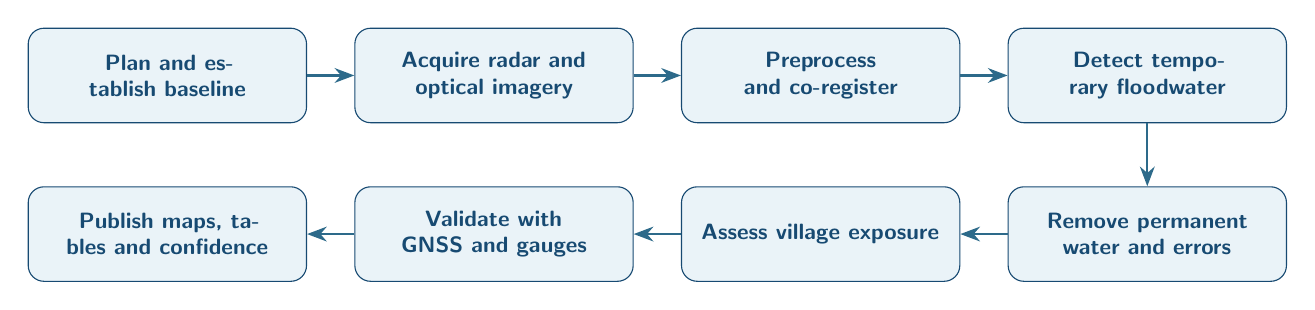
\begin{tikzpicture}[node distance=8mm and 6mm]
\node[flownode] (baseline) {Plan and establish baseline};
\node[flownode, right=of baseline] (acquire) {Acquire radar and optical imagery};
\node[flownode, right=of acquire] (preprocess) {Preprocess and co-register};
\node[flownode, right=of preprocess] (detect) {Detect temporary floodwater};
\node[flownode, below=of detect] (errors) {Remove permanent water and errors};
\node[flownode, left=of errors] (assess) {Assess village exposure};
\node[flownode, left=of assess] (validate) {Validate with GNSS and gauges};
\node[flownode, left=of validate] (publish) {Publish maps, tables and confidence};
\draw[flowarrow] (baseline) -- (acquire);
\draw[flowarrow] (acquire) -- (preprocess);
\draw[flowarrow] (preprocess) -- (detect);
\draw[flowarrow] (detect) -- (errors);
\draw[flowarrow] (errors) -- (assess);
\draw[flowarrow] (assess) -- (validate);
\draw[flowarrow] (validate) -- (publish);
\end{tikzpicture}
\caption{End-to-end flood-inundation mapping workflow from event definition to confidence-aware publication.}
\label{fig:flood-mapping-workflow}
\end{figure}

\subsection{Step 1 - Define the event, area and output standard}\label{step-1---define-the-event-area-and-output-standard}

\begin{quote}
1. Record the rainfall period, expected flood peak, satellite acquisition window and district boundary.

2. Select a common projected coordinate reference system suitable for area calculations, normally the relevant UTM zone or an official state projection.

3. Define the minimum mapping unit, for example 0.25-1 ha for medium-resolution mapping, and specify whether shallow water, flooded vegetation and urban flooding are included.

4. Define the affected-village severity rule before processing to avoid changing criteria after seeing results.
\end{quote}

\subsection{Step 2 - Assemble reference and exposure layers}\label{step-2---assemble-reference-and-exposure-layers}

\begin{itemize}
\item
  District, block, taluk and village boundaries from an authoritative administrative source.
\item
  River network, tanks, reservoirs, canals, wetlands and a permanent-water mask.
\item
  Digital elevation model, slope, flow accumulation and, where possible, Height Above Nearest Drainage (HAND).
\item
  Roads, bridges, railways, buildings, schools, health centres, substations, shelters and critical facilities.
\item
  Population, settlement and crop/land-use layers for exposure estimation.
\item
  Rain-gauge, river-stage, reservoir-release and GNSS field-observation data.
\end{itemize}

\subsection{Step 3 - Select pre-flood and post-flood satellite scenes}\label{step-3---select-pre-flood-and-post-flood-satellite-scenes}

Choose a recent pre-flood image representing normal conditions and the earliest useful post-flood image. For Sentinel-1, match orbit direction, relative orbit, acquisition mode and polarization whenever possible. Using comparable geometry minimizes false change caused by incidence angle, surface moisture or viewing direction. If a single post-event acquisition is unavailable, use a time series and identify the maximum observed flood extent.

\subsection{Step 4 - Preprocess SAR imagery}\label{step-4---preprocess-sar-imagery}

\begin{quote}
1. Apply precise orbit information.

2. Remove border noise and thermal noise when required by the product and software.

3. Radiometrically calibrate to sigma nought or gamma nought backscatter.

4. Apply a conservative speckle filter or multi-temporal filter; avoid excessive smoothing of narrow channels and village-scale features.

5. Terrain-correct the image using a DEM and resample to a consistent pixel size.

6. Convert backscatter to decibels (dB) for interpretation and thresholding.

7. Co-register pre- and post-event images precisely for pixel-wise change detection.
\end{quote}

\subsection{Step 5 - Extract potential floodwater}\label{step-5---extract-potential-floodwater}

Use at least two complementary indicators rather than one global threshold. First, identify low post-event backscatter that is characteristic of smooth open water. Second, calculate change between pre- and post-event images, such as a dB difference or backscatter ratio. A pixel is more likely to be temporary floodwater when it was non-water before the event, becomes dark after the event, lies on plausible low-relief terrain and connects to a drainage or known floodplain.

\begin{itemize}
\item
  Single-date method: classify post-event SAR using global or local thresholding.
\item
  Change method: classify significant pre/post backscatter decrease, then combine with the single-date water mask.
\item
  Dual-polarization method: use VV, VH and their ratio/difference as classifier features.
\item
  Machine-learning method: train Random Forest, gradient boosting or a validated deep model using water, non-water, urban, vegetation and shadow samples.
\end{itemize}

\subsection{Step 6 - Process optical imagery for confirmation}\label{step-6---process-optical-imagery-for-confirmation}

\begin{quote}
1. Use atmospherically corrected surface-reflectance products where possible.

2. Mask cloud, cirrus and cloud shadow using quality bands or a cloud-probability product.

3. Calculate NDWI, MNDWI and/or AWEI and classify water using scene-specific thresholds.

4. Compare optical water with SAR results; retain agreement as high confidence and inspect disagreements.

5. Use false-colour composites to interpret sediment-rich water, vegetation, soil moisture and built-up areas.
\end{quote}

\subsection{Step 7 - Remove permanent water and probable false positives}\label{step-7---remove-permanent-water-and-probable-false-positives}

Subtract a permanent-water layer or pre-event water mask so the final layer represents temporary inundation. Exclude implausible steep slopes and isolated pixels that are disconnected from floodplain terrain, unless field evidence shows local ponding or landslide-dammed water. Create separate masks for radar shadow, cloud, cloud shadow and no-data areas so that uncertainty is visible rather than silently treated as dry land.

\subsection{Step 8 - Post-process and vectorize}\label{step-8---post-process-and-vectorize}

\begin{itemize}
\item
  Apply morphological opening/closing to remove isolated noise and fill small gaps.
\item
  Use connected-component analysis and a minimum-area filter.
\item
  Preserve narrow water connections where they represent real channels or road overtopping.
\item
  Convert the cleaned raster to polygons, repair geometry and calculate area in hectares or square kilometres.
\item
  Attach acquisition time, sensor, method, confidence and processing version to the output metadata.
\end{itemize}

\subsection{Step 9 - Identify and rank affected villages}\label{step-9---identify-and-rank-affected-villages}

Intersect the temporary flood polygon with village boundaries and calculate the following attributes for each village:

\begin{itemize}
\item
  Flooded area (ha) and percentage of village area.
\item
  Flooded built-up area, crop area and critical-facility count.
\item
  Length of affected road and number of potentially cut road links or bridges.
\item
  Estimated exposed population, with an explicit note that exposure is not the same as confirmed affected population.
\item
  Maximum or modelled flood depth, when a hydraulic surface is available.
\item
  Confidence score based on sensor agreement, terrain consistency and field validation.
\end{itemize}

\begin{longtable}{|
  >{\raggedright\arraybackslash}p{(\columnwidth - 6\tabcolsep - 4\arrayrulewidth) * \real{0.18}}|
  >{\raggedright\arraybackslash}p{(\columnwidth - 6\tabcolsep - 4\arrayrulewidth) * \real{0.39}}|
  >{\raggedright\arraybackslash}p{(\columnwidth - 6\tabcolsep - 4\arrayrulewidth) * \real{0.43}}|}
\hline
\rowcolor{LightBlue}
\textbf{\sffamily Severity} &
\textbf{\sffamily Suggested rule} &
\textbf{\sffamily Administrative interpretation} \\ \hline
\endhead
\hline
\endfoot
\hline
\endlastfoot
\textbf{Very High} & \textgreater25\% village inundated, or major settlement/critical facility/primary access route affected & Immediate verification, rescue readiness and evacuation decision. \\ \hline
\textbf{High} & 10-25\% inundated or multiple assets/crop clusters affected & Priority relief, road-access assessment and field team deployment. \\ \hline
\textbf{Moderate} & 2-10\% inundated or localized asset exposure & Targeted monitoring and local warning. \\ \hline
\textbf{Low} & \textless2\% inundated with no confirmed asset impact & Verify; may be peripheral floodplain or mapping noise. \\ \hline
\textbf{Uncertain} & Cloud, radar shadow, no data, disagreement or no field confirmation & Do not label safe; prioritize additional observation. \\ \hline
\end{longtable}

Table 2. Example severity rules. Thresholds should be calibrated to local geography, village size and district response capacity.

The UNOSAT product in Figure~\ref{fig:unosat-pakistan} shows how detected floodwater can be translated into an operational map that combines inundation extent, administrative context, settlements, roads, before-and-after imagery and an estimate of potentially exposed population. It also labels the analysis as preliminary and requests field validation, matching the confidence-aware workflow recommended in this assignment.

\begin{landscape}
\thispagestyle{fancy}
\begin{figure}[H]
\centering
\includegraphics[width=0.82\linewidth]{unosat_pakistan_flood_map.jpg}
\caption{Satellite-detected floodwater and potential population exposure across parts of Pakistan as of 1 July 2025. The product combines Sentinel-2-derived water extent with settlements, boundaries, transport, population estimates and before/after image insets. Credit: United Nations Satellite Centre (UNOSAT); contains modified Copernicus Sentinel data (2025) {[}16{]}.}
\label{fig:unosat-pakistan}
\end{figure}
\end{landscape}

\subsection{Step 10 - Validate accuracy and publish outputs}\label{step-10---validate-accuracy-and-publish-outputs}

Select validation samples using stratified random sampling across mapped water, dry land, urban areas, vegetation and uncertain zones. Use high-resolution imagery, GNSS-tagged photographs, drone observations where permitted, gauge records and local administrative reports. Calculate a confusion matrix, overall accuracy, user accuracy, producer accuracy, precision, recall and F1-score for the flood class. Report omission errors separately because missed flooded villages may have greater operational consequences than small false-positive areas.

\begin{itemize}
\item
  Flood extent map with date, time, sensor, legend, scale, north arrow, source and uncertainty mask.
\item
  Affected-village spreadsheet/table with severity and exposure indicators.
\item
  Safe access, shelter and critical-facility map for field operations.
\item
  Web GIS dashboard showing latest extent, previous extent, gauges, alerts and field reports.
\item
  Processing log and metadata so the result can be audited and updated.
\end{itemize}

\section{5. Image-Processing Techniques to Improve Flood Detection Accuracy}\label{image-processing-techniques-to-improve-flood-detection-accuracy}

\subsection{5.1 SAR-specific techniques}\label{sar-specific-techniques}

\subsubsection{Radiometric calibration and terrain correction}\label{radiometric-calibration-and-terrain-correction}

Calibration converts digital values to physically meaningful backscatter, while terrain correction removes geometric displacement caused by side-looking radar and topography. Without these steps, thresholds may vary across the scene and flood polygons may not align with village or road layers.

\subsubsection{Speckle reduction without destroying edges}\label{speckle-reduction-without-destroying-edges}

SAR speckle is a multiplicative noise pattern. Refined Lee, Lee Sigma, Gamma-MAP or multi-temporal filters can stabilize water classification. A small window is preferred for village-scale mapping; aggressive filtering can erase narrow flood channels or merge water with adjacent dark surfaces.

\subsubsection{Adaptive thresholding}\label{adaptive-thresholding}

A single backscatter threshold is simple but may fail across different soils, incidence angles and land-cover types. Otsu thresholding {[}13{]}, histogram valley detection, local adaptive thresholds or terrain-stratified thresholds should be tested. Thresholds must be validated for each event rather than copied blindly from another region.

\subsubsection{Multi-temporal change detection}\label{multi-temporal-change-detection}

Subtracting or ratioing post-event and pre-event backscatter helps isolate newly inundated areas from permanent dark surfaces. A robust rule can require both low post-event backscatter and a significant decrease from baseline. Median or percentile composites from several pre-event dates are better than one baseline scene because they reduce effects of agricultural moisture and sensor noise.

\subsubsection{Polarization and texture features}\label{polarization-and-texture-features}

VV and VH respond differently to surface roughness and vegetation. Combining VV, VH, VV/VH ratio, local mean, standard deviation and texture measures improves separation of open water, wet soil, crops and built-up areas. In flooded vegetation and urban areas, double-bounce scattering may increase backscatter; a dark-water-only rule will miss these zones.

\subsubsection{Coherence and object-based methods}\label{coherence-and-object-based-methods}

Interferometric coherence can decrease when the surface changes between acquisitions and may support flood detection when suitable image pairs are available. Object-based image analysis groups neighbouring pixels into meaningful regions and can reduce salt-and-pepper noise, especially when combined with shape, terrain and connectivity rules.

\subsection{5.2 Optical-image techniques}\label{optical-image-techniques}

\subsubsection{Cloud and shadow masking}\label{cloud-and-shadow-masking}

Reliable cloud, cirrus and cloud-shadow masks are mandatory. Cloud shadow is often dark and can be falsely classified as water. Suspect areas should be labelled uncertain or replaced with SAR evidence, not treated as confirmed dry or flooded.

\subsubsection{Water indices}\label{water-indices}

Common spectral indices include:

\begin{itemize}
\item
  NDWI = (Green - NIR) / (Green + NIR), originally proposed for open-water enhancement {[}10{]}.
\item
  MNDWI = (Green - SWIR) / (Green + SWIR), which often suppresses built-up surfaces more effectively {[}11{]}.
\item
  AWEI combines visible, NIR and SWIR bands to improve water extraction in shadowed and dark-surface conditions {[}12{]}.
\end{itemize}

No index has a universal threshold. Scene-specific thresholding, histogram inspection and reference samples are required. MNDWI may work well in built-up areas, while NDWI or AWEI may perform better in other land-cover conditions.

\subsubsection{Atmospheric correction and compositing}\label{atmospheric-correction-and-compositing}

Use surface-reflectance products, consistent band scaling and quality masks. A multi-date minimum-NIR or maximum-water composite can reduce cloud gaps, but the composite date must be documented because it may combine different flood stages.

\subsection{5.3 Multi-source data fusion}\label{multi-source-data-fusion}

The strongest accuracy improvement usually comes from combining independent evidence rather than tuning one threshold. A practical confidence model can assign higher confidence where SAR, optical indices, low elevation, drainage connectivity and rainfall/gauge observations agree.

\begin{longtable}{|
  >{\raggedright\arraybackslash}p{(\columnwidth - 6\tabcolsep - 4\arrayrulewidth) * \real{0.34}}|
  >{\raggedright\arraybackslash}p{(\columnwidth - 6\tabcolsep - 4\arrayrulewidth) * \real{0.38}}|
  >{\raggedright\arraybackslash}p{(\columnwidth - 6\tabcolsep - 4\arrayrulewidth) * \real{0.28}}|}
\hline
\rowcolor{LightBlue}
\textbf{\sffamily Evidence} &
\textbf{\sffamily Example interpretation} &
\textbf{\sffamily Use in confidence score} \\ \hline
\endhead
\hline
\endfoot
\hline
\endlastfoot
\textbf{SAR low backscatter + strong decrease} & New smooth open water is likely & High positive evidence \\ \hline
\textbf{Optical MNDWI/AWEI water} & Spectral response supports water & Positive confirmation \\ \hline
\textbf{Low HAND / near drainage} & Hydrologically plausible floodplain & Positive contextual evidence \\ \hline
\textbf{Permanent-water occurrence} & Normal river/tank/lake, not temporary flood & Subtract or classify separately \\ \hline
\textbf{Steep slope / radar shadow} & Likely false positive or uncertain & Penalty or uncertainty flag \\ \hline
\textbf{GNSS photo / gauge exceedance} & Ground confirmation & Very high confidence \\ \hline
\textbf{Sensor disagreement} & Possible vegetation, urban flooding, cloud or timing difference & Manual review / uncertain \\ \hline
\end{longtable}

Table 3. Evidence-fusion logic for confidence-aware flood mapping.

\subsection{5.4 Machine learning and deep learning}\label{machine-learning-and-deep-learning}

Random Forest is a strong operational baseline because it handles nonlinear relationships, mixed feature scales and limited training data, and it provides feature importance. Gradient boosting can improve discrimination but requires careful tuning. Convolutional neural networks and transformer-based segmentation models can map complex flooded vegetation and urban patterns, but they require representative training data, rigorous validation and transfer testing across seasons and districts. A model with high average accuracy may still fail during a new flood if sensor geometry, crop stage or urban structure differs from the training set.

\subsection{5.5 Recommended accuracy-control measures}\label{recommended-accuracy-control-measures}

\begin{itemize}
\item
  Use independent validation data and avoid validating with the same samples used for training or threshold selection.
\item
  Report confidence/uncertainty alongside the binary flood map.
\item
  Maintain separate classes for permanent water, temporary floodwater, uncertain, cloud/no-data and radar shadow.
\item
  Test sensitivity to threshold changes and minimum mapping unit.
\item
  Compare results with river stage, rainfall timing and known topography; implausible isolated high-slope water should be reviewed.
\item
  Version every map and retain the input-scene identifiers and processing settings.
\end{itemize}

\section{6. Early-Warning Framework Integrating Satellite Imagery, GNSS and GIS}\label{early-warning-framework-integrating-satellite-imagery-gnss-and-gis}

An effective early-warning system must cover the entire chain from risk knowledge to observation, forecasting, warning communication and response. Satellite imagery alone is normally an observation after or during inundation; therefore, it should be combined with rainfall forecasts, satellite precipitation, river gauges, reservoir data and hydrologic/hydraulic models to provide lead time.

\begin{figure}[H]
\centering
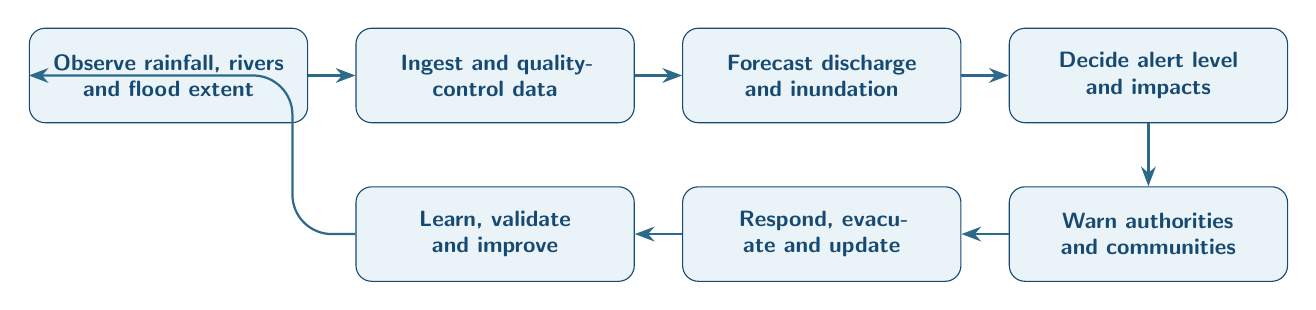
\begin{tikzpicture}[node distance=8mm and 6mm]
\node[flownode] (observe) {Observe rainfall, rivers and flood extent};
\node[flownode, right=of observe] (ingest) {Ingest and quality-control data};
\node[flownode, right=of ingest] (forecast) {Forecast discharge and inundation};
\node[flownode, right=of forecast] (decide) {Decide alert level and impacts};
\node[flownode, below=of decide] (warn) {Warn authorities and communities};
\node[flownode, left=of warn] (respond) {Respond, evacuate and update};
\node[flownode, left=of respond] (learn) {Learn, validate and improve};
\draw[flowarrow] (observe) -- (ingest);
\draw[flowarrow] (ingest) -- (forecast);
\draw[flowarrow] (forecast) -- (decide);
\draw[flowarrow] (decide) -- (warn);
\draw[flowarrow] (warn) -- (respond);
\draw[flowarrow] (respond) -- (learn);
\draw[flowarrow, rounded corners=5mm] (learn.west) -- ++(-8mm,0) |- (observe.west);
\end{tikzpicture}
\caption{Seven-stage integrated flood early-warning cycle with a feedback loop from response evaluation to renewed observation.}
\label{fig:early-warning-cycle}
\end{figure}

\subsection{6.1 Observation layer}\label{observation-layer}

\begin{itemize}
\item
  Weather satellites and radar: INSAT imagery, IMD radar products and satellite rainfall estimates for cloud development, rainfall intensity and accumulation.
\item
  Earth-observation satellites: Sentinel-1/EOS-04-type SAR for all-weather flood extent; Sentinel-2/Landsat for cloud-free confirmation and land-impact mapping.
\item
  Ground sensors: automatic rain gauges, river-stage gauges, reservoir inflow/outflow and soil-moisture sensors.
\item
  GNSS: precise coordinates and timestamps for gauges, field photos, water marks, road closures, rescue teams, shelters and mobile survey observations. GNSS provides global positioning and timing to receivers {[}8{]}.
\item
  Community observations: geotagged reports from village officers, police, fire and rescue, health workers and trained volunteers.
\end{itemize}

\subsection{6.2 Data-ingestion and GIS platform}\label{data-ingestion-and-gis-platform}

All feeds should enter a common spatial database with standardized coordinate systems, timestamps, sensor identifiers and quality flags. Automated scripts should download or receive new rainfall, gauge and satellite products, trigger preprocessing, and publish time-enabled layers to a secure district GIS dashboard. The dashboard should show current rainfall, forecast rainfall, river levels, reservoir releases, flood probability, detected water, affected villages, shelters, road closures and field-team locations.

\subsection{6.3 Forecast and inundation modelling}\label{forecast-and-inundation-modelling}

\begin{itemize}
\item
  Rainfall-runoff modelling converts observed and forecast rainfall into catchment discharge.
\item
  River-routing and two-dimensional hydraulic models estimate water level, depth, velocity and likely inundation for forecast discharges.
\item
  DEM, drainage, embankments, culverts and land-cover roughness should be updated because model accuracy depends strongly on terrain and infrastructure representation.
\item
  Satellite flood extents calibrate or correct modelled inundation during the event, creating a data-assimilation loop.
\end{itemize}

\subsection{6.4 Alert decision logic}\label{alert-decision-logic}

Use both threshold-based and impact-based triggers. A simple three-level framework is:

\begin{longtable}{|
  >{\raggedright\arraybackslash}p{(\columnwidth - 6\tabcolsep - 4\arrayrulewidth) * \real{0.20}}|
  >{\raggedright\arraybackslash}p{(\columnwidth - 6\tabcolsep - 4\arrayrulewidth) * \real{0.40}}|
  >{\raggedright\arraybackslash}p{(\columnwidth - 6\tabcolsep - 4\arrayrulewidth) * \real{0.40}}|}
\hline
\rowcolor{LightBlue}
\textbf{\sffamily Level} &
\textbf{\sffamily Illustrative trigger} &
\textbf{\sffamily Action} \\ \hline
\endhead
\hline
\endfoot
\hline
\endlastfoot
\textbf{Watch} & Heavy rainfall forecast/observed; catchment saturation; river rising but below danger level & Activate control room, verify sensors, pre-position teams, monitor vulnerable villages. \\ \hline
\textbf{Warning} & River or reservoir threshold exceeded; model predicts village/road exposure; satellite rainfall persists & Issue public warning, open shelters, restrict unsafe routes, deploy field verification. \\ \hline
\textbf{Evacuation / Emergency} & Observed or forecast dangerous depth/velocity; critical access cut; GNSS field report or satellite map confirms rapid spread & Evacuate priority zones, dispatch rescue, isolate power/traffic hazards and update continuously. \\ \hline
\end{longtable}

Table 4. Illustrative alert levels. Legal thresholds and public messaging must follow state and district disaster-management protocols.

\subsection{6.5 Warning dissemination}\label{warning-dissemination}

Warnings should use redundant channels: cell broadcast/SMS, official mobile apps, sirens, public-address systems, television/radio, social media, police and local-government networks. Messages should identify the affected place, hazard, expected time, required action, safe route or shelter, issuing authority and update time. A Common Alerting Protocol-compatible structure improves consistency across channels.

\subsection{6.6 GNSS-enabled field response and validation}\label{gnss-enabled-field-response-and-validation}

Mobile teams should use a standardized form that captures latitude, longitude, time, water depth, flow condition, road status, photograph, source and confidence. Offline-capable forms are important because connectivity may fail. GNSS positions can update road closures, confirm flood edges, guide rescue teams and validate the next satellite map. Safety rules must prevent teams from entering fast-flowing or electrically hazardous areas merely to collect data.

\subsection{6.7 Feedback and continuous improvement}\label{feedback-and-continuous-improvement}

After each event, compare forecasts, modelled extent, satellite extent and GNSS observations. Record missed villages, false alarms, communication delays, sensor failures and evacuation outcomes. Update thresholds, training data, terrain layers, contact lists and standard operating procedures before the next monsoon. UNOSAT operational products demonstrate how satellite-detected floodwater can be combined with exposure layers, while also noting that preliminary satellite analyses require ground validation {[}9{]}.

\section{7. Recommended District Implementation Plan}\label{recommended-district-implementation-plan}

\subsection{7.1 Phase 1 - Preparedness before the monsoon}\label{phase-1---preparedness-before-the-monsoon}

\begin{itemize}
\item
  Create a single authoritative geodatabase for village boundaries, rivers, tanks, drainage, roads, bridges, buildings, critical facilities and shelters.
\item
  Prepare pre-event Sentinel-1 backscatter composites and optical permanent-water masks for the entire district.
\item
  Precompute DEM derivatives: slope, flow accumulation, sub-basins, floodplain/HAND and low-lying settlement zones.
\item
  Define alert thresholds with irrigation, revenue, police, fire, health and local-government departments.
\item
  Prepare QGIS project templates, processing models, map layouts and affected-village report formats.
\item
  Train field teams in GNSS data collection, safety, photo standards and offline synchronization.
\end{itemize}

\subsection{7.2 Phase 2 - During heavy rainfall}\label{phase-2---during-heavy-rainfall}

\begin{itemize}
\item
  Monitor forecast rainfall, satellite precipitation, radar, gauges and reservoir releases continuously.
\item
  Generate forecast impact layers before the satellite overpass and issue watches/warnings when thresholds are reached.
\item
  Acquire and process the first available SAR scene; publish a preliminary map with confidence and no-data layers.
\item
  Prioritize uncertain villages and high-impact assets for GNSS field verification.
\item
  Update the map whenever a new satellite scene, gauge reading or validated field report arrives.
\end{itemize}

\subsection{7.3 Phase 3 - Recovery and assessment}\label{phase-3---recovery-and-assessment}

\begin{itemize}
\item
  Map maximum observed flood extent and duration using all available dates.
\item
  Estimate crop, road, building and public-infrastructure exposure; keep exposure estimates separate from verified damage.
\item
  Archive the event database, processing chain, maps and field observations.
\item
  Conduct an after-action review and revise models, thresholds and vulnerable-village lists.
\end{itemize}

\subsection{7.4 Suggested technology stack}\label{suggested-technology-stack}

\begin{longtable}{|
  >{\raggedright\arraybackslash}p{(\columnwidth - 4\tabcolsep - 3\arrayrulewidth) * \real{0.34}}|
  >{\raggedright\arraybackslash}p{(\columnwidth - 4\tabcolsep - 3\arrayrulewidth) * \real{0.66}}|}
\hline
\rowcolor{LightBlue}
\textbf{\sffamily Function} &
\textbf{\sffamily Suggested tools/data} \\ \hline
\endhead
\hline
\endfoot
\hline
\endlastfoot
\textbf{Satellite preprocessing} & ESA SNAP for Sentinel-1; QGIS Processing/GDAL; Python/rasterio where automation is required. \\ \hline
\textbf{GIS analysis and cartography} & QGIS with GeoPackage/PostGIS, zonal statistics, raster calculator, overlay and print layouts. \\ \hline
\textbf{Database and dashboard} & PostGIS plus GeoServer/QGIS Server or a secured equivalent; time-enabled web map/dashboard. \\ \hline
\textbf{Field data} & GNSS-enabled phones/tablets with offline forms; differential GNSS for critical control points if available. \\ \hline
\textbf{Models} & A calibrated rainfall-runoff model and HEC-RAS 2D or an equivalent hydraulic model. \\ \hline
\textbf{Data sources} & Copernicus Data Space, USGS EarthExplorer, ISRO/NRSC/Bhuvan operational channels, IMD, CWC/state gauges and local departments. \\ \hline
\end{longtable}

\section{8. Limitations, Quality Assurance and Conclusion}\label{limitations-quality-assurance-and-conclusion}

\subsection{8.1 Quality-assurance checklist}\label{quality-assurance-checklist}

\begin{quote}
$\square$ Are the pre- and post-event scenes geometrically aligned and comparable?

$\square$ Were SAR calibration, terrain correction and optical cloud masking completed correctly?

$\square$ Was permanent water separated from temporary inundation?

$\square$ Are radar shadow, cloud/no-data and uncertain zones visible?

$\square$ Were steep-slope and implausible isolated detections reviewed?

$\square$ Were affected-village rules defined consistently and area calculations performed in an appropriate projected CRS?

$\square$ Was accuracy assessed using independent field or high-resolution reference data?

$\square$ Does the map show acquisition time, source, processing version, confidence and limitations?

$\square$ Are exposure estimates clearly distinguished from verified damage and confirmed affected population?

$\square$ Were warnings approved and disseminated through authorized disaster-management procedures?
\end{quote}

\subsection{8.2 Conclusion}\label{conclusion}

Satellite imagery provides a fast, consistent and wide-area basis for mapping floods, but its greatest administrative value emerges only after GIS analysis converts water extent into village-level impact information. For rainfall-driven emergencies, SAR imagery should be the operational foundation because it is not blocked by cloud or darkness. Optical imagery, long-term archives, meteorological satellites, elevation data, gauges and GNSS observations should be fused to improve interpretation and reduce false classifications.

The proposed workflow begins with comparable pre- and post-event imagery, performs sensor-specific preprocessing, applies thresholding or classification and change detection, removes permanent water and terrain-related errors, intersects the cleaned flood layer with village and exposure data, validates the result, and publishes confidence-aware products. The early-warning framework extends this approach upstream in time by combining rainfall and river monitoring with hydrologic/hydraulic forecasting, threshold-based alerts, GIS dashboards and GNSS-enabled field feedback. This integrated method enables the district administration to move from reactive flood mapping toward anticipatory, evidence-based warning and response.

\begin{summarybox}
{\sffamily\bfseries\color{Primary}Final recommendation}\par
Adopt a multi-sensor, confidence-aware workflow. Do not issue a village-level declaration from one unvalidated image. Use radar, optical, terrain, gauges and GNSS evidence together, and update the operational map as new observations arrive.
\end{summarybox}

\section{References}\label{references}

\begin{quote}
\textbf{{[}1{]} European Space Agency (ESA).} Sentinel-1: Facts and Figures; Sentinel-1 Instrument. All-weather/day-night SAR, IW swath and resolution, and nominal revisit information. \href{https://www.esa.int/Applications/Observing_the_Earth/Copernicus/Sentinel-1/Facts_and_figures}{Online source}

\textbf{{[}2{]} European Space Agency (ESA).} Sentinel-2 mission overview. Spatial resolution, spectral bands, swath and revisit. \href{https://www.esa.int/Applications/Observing_the_Earth/Copernicus/Sentinel-2}{Online source}

\textbf{{[}3{]} U.S. Geological Survey (USGS).} Landsat 8-9 OLI/TIRS Collection 2 Level-1 Data and Landsat 8 mission characteristics. \href{https://www.usgs.gov/centers/eros/science/usgs-eros-archive-landsat-archives-landsat-8-9-operational-land-imager-and}{Online source}

\textbf{{[}4{]} National Aeronautics and Space Administration (NASA).} MODIS Data: swath, temporal coverage, spectral bands and spatial resolutions. \href{https://modis.gsfc.nasa.gov/data/}{Online source}

\textbf{{[}5{]} NASA Earthdata.} Near Real-Time Global Flood Products from MODIS and VIIRS. \href{https://www.earthdata.nasa.gov/data/instruments/viirs/near-real-time-data/nrt-global-flood-products}{Online source}

\textbf{{[}6{]} Indian Space Research Organisation (ISRO).} EOS-04 radar imaging satellite: all-weather imaging and flood-mapping application. \href{https://www.isro.gov.in/mission_PSLV_C52_EOS_04.html}{Online source}

\textbf{{[}7{]} Indian Space Research Organisation (ISRO).} INSAT-3DS mission: meteorological observations, weather forecasting and disaster warning. \href{https://www.isro.gov.in/GSLV-F14_INSAT-3DS_mission.html}{Online source}

\textbf{{[}8{]} United Nations Office for Outer Space Affairs (UNOOSA).} Global Navigation Satellite Systems: positioning and timing principles and applications. \href{https://www.unoosa.org/oosa/en/ourwork/psa/gnss/gnss.html}{Online source}

\textbf{{[}9{]} United Nations Satellite Centre (UNOSAT).} Operational flood mapping products and exposure analysis using satellite-detected water. \href{https://unosat.org/}{Online source}

\textbf{{[}10{]} McFeeters, S. K. (1996).} The use of the Normalized Difference Water Index (NDWI) in the delineation of open water features. International Journal of Remote Sensing, 17(7), 1425-1432. \href{https://doi.org/10.1080/01431169608948714}{Online source}

\textbf{{[}11{]} Xu, H. (2006).} Modification of Normalised Difference Water Index (NDWI) to enhance open water features in remotely sensed imagery. International Journal of Remote Sensing, 27(14), 3025-3033. \href{https://doi.org/10.1080/01431160600589179}{Online source}

\textbf{{[}12{]} Feyisa, G. L., Meilby, H., Fensholt, R., \& Proud, S. R. (2014).} Automated Water Extraction Index: A new technique for surface water mapping using Landsat imagery. Remote Sensing of Environment, 140, 23-35. \href{https://doi.org/10.1016/j.rse.2013.08.029}{Online source}

\textbf{{[}13{]} Otsu, N. (1979).} A threshold selection method from gray-level histograms. IEEE Transactions on Systems, Man, and Cybernetics, 9(1), 62-66. \href{https://doi.org/10.1109/TSMC.1979.4310076}{Online source}

\textbf{{[}14{]} ESA STEP.} Sentinel-1 Flood Mapping Tutorial. \href{https://step.esa.int/docs/tutorials/tutorial_s1floodmapping.pdf}{Online source}

\textbf{{[}15{]} European Space Agency (ESA).} Sentinel-1 derived map of flood-affected urban area, Valencia, Spain, 31 October 2024. Contains modified Copernicus Sentinel data (2024), produced by ESA/LIST. \href{https://www.esa.int/ESA_Multimedia/Images/2024/11/Sentinel-1_derived_map_of_flood_affected_urban_area_-_Valencia_Spain}{Online source}

\textbf{{[}16{]} United Nations Satellite Centre (UNOSAT).} Satellite-detected water extents in Sindh, Balochistan and Punjab Provinces, Pakistan, as of 1 July 2025. Product 4142; contains modified Copernicus Sentinel data (2025). \href{https://unosat.org/products/4142}{Online source}
\end{quote}
\end{document}
